\chapter{Introduction}
\section{Streszczenie}
    W poniższej pracy inżynierskiej przedstawiono proces tworzenia narzędzia do wyceny wybranych instrumentów finansowych. Zaprezentowano wycenę europejskiej opcji przy użyciu znanego modelu Blacka-Scholes'a z 1973 roku, gdzie instrumentem podstawowym jest akcja wygenerowana za pomocą Geometrycznego Rruchu Browna. Pokazano również zastosowanie modelu Black'a z 1976 roku, gdzie w przeciwieństwie do poprzedniego modelu cena instrumentu bazowego zostaje zastąpiona zdyskontowaną wartością kontraktu futures/forward na ten instrument.
    
    W tym celu została stworzona aplikacja desktopowa w języku F\#, w paradygmacie programowania funkcyjnego, przy użyciu wzorca MVVM oraz technologii XAML do stworzenia interfejsu użytkownika. Aplikacja nosi nazwę MARS App -- jest to akronim od angielskiego \textit{Market And Risk Simulation Application}, co oznacza aplikację przeznaczoną do symulacji rynku i ryzka. Praca zawiera również swoisty poradnik, jak stworzyć aplikację w języku F\#, opartą o architekturę MVVM w zintegrowanym środowisku programistycznym Visual Studio 2019 będącym produktem firmy Microsoft, ponieważ dokładnie powyższe połączenie różnych technologii nie jest bardzo często spotykane, co przejawia się zredukowaną ilością poradników pomagających stworzyć podobną aplikację nowym użytkownikom.
    
    \emph{Słowa kluczowe: programowanie funkcyjne, instrumenty finansowe, wycena, MVVM, Black-Scholes, Black}

\section{Abstract}
    This paper is an overview of some methods used for pricing selected financial instruments (or their derivatives). Main part of the project was creating a tool - computer program written mostly in F\# for that purpose. The application is named \textit{MARS App} -- it is an acronym  of the English words \textit{Market And Risk Simulation}. Two models have been presented: first being Black-Scholes model from 1973 which gives an estimate of the price of european-style option. As the underlying asset stock price was used. In order to generate stock prices over time Geometric Brownion Motion has been implemented as this stochastic process is usually applied in the Black-Scholes model. The other model is Black's model from 1976 which is a slightly altered Black-Scholes model while it is adjusted for valuing options on futures contracts.
    
    This paper can be as well kind of a guide how to create an F\# application using MVVM architecture with XAML markup language for creating user interface as such tutorials are scarce in literature.
    
    \emph{Keywords: functional programming, financial instruments, pricing, MVVM, Black-Scholes, Black}

\section{Thesis assumptions}
    The main goal is to create a tool in functional programming paradigm which will be used to price selected financial instruments. To achieve this goal F\# programming language will be used as it was created mostly to support functional programming and European option will be priced as an example of a derivative financial instrument.
    %
    App will consist of several different technologies such as MVVM design pattern, XAML language to create View part of the project and minor C\# background to connect XAML's View with F\#'s ViewModel. Everything will be written in Visual Studio 2019 IDE.
    
    Basic assumptions within the application include:
    \begin{itemize}
        \item \textit{Geometric Brownian Motion} implementation as a model used for generating underlying asset prices.
        \item Ability to specialize the product by changing:
            \begin{itemize}
                \item maturity (expiration time),
                \item interest rate,
                \item stock's initial price,
                \item drift,
                \item volatility.
            \end{itemize}
        \item Implementing Black-Scholes model for option pricing.
        \item Preparation of the application's graphic design in XAML and connecting the View with logic.
    \end{itemize}

% \section{Scope of the thesis}
%     \todo{fill in at the end}
%     In chapter 1 - blabla
%     In chapter 2 I will talk about blablah

\section{Technologies Overview}
\subsection{Programming paradigms}
    Programming paradigm is nothing more but an overall concept which describes \textit{how} the programming is done and what is the methodology behind the language that adheres to a specific type of a paradigm. Throughout the years programming languages evolved, new ones have been created, so that today there are from 150, according to TIOBE Programming Community, up to 700, listed by Wikipedia, different programming languages (more information can be found here \cite{numberOfProgrammingLanguages}). Although some sources (see here \cite{numberOfProgrammingLanguages_hopl_info}) state that there are almost as many as 9000 (sic) programming languages the exact number of those is not that important -- rather variety and the fact that there are many of them is crucial as it indicates that they must differ from each other and it turns out these differences can somehow be grouped, what is presented below.
    
    The most basic and intuitive approach into dividing paradigms is into 2 groups:
    \begin{itemize}
        \item Imperative Programming
        \item Declarative Programming
    \end{itemize}
    
    \subsubsection{Imperative Programming}
    This way of programming is not by accident described as the first one -- historically languages that present this type of programming have emerged primarily. Imperative programming enables the programmer to manage processor's behaviour on much more precise level. Commands show step-by-step how the computation is executed. These commands affect a program's state. This paradigm focuses on describing \textit{how} the goal should be achieved.
    
    Imperative programming can be further broken down into 3 groups:
    \begin{enumerate}
        \item \textbf{Procedural Programming} -- underlying model is based on a procedure (set of coded instructions, more detail here \cite{procedureDefinition}). It has the ability to reuse code written once. Examples of procedural programming languages:
            \begin{itemize}
                \item C,
                \item C++,
                \item Java,
                \item ColdFusion,
                \item Pascal.
            \end{itemize}
        \item \textbf{Object Oriented Programming} -- program is a set of classes and objects (instances of a class) that are meant to interact with each other. Examples of languages supporting OOP paradigm:
            \begin{itemize}
                \item Objective-C,
                \item C++,
                \item Java,
                \item Visual Basic .NET,
                \item Python.
            \end{itemize}
        \item \textbf{Parallel Processing Approach} -- this style of programming is designed to divide computing the code into multiple processors in order to minimize time required for computation. Example of languages supporting parallel programming approach:
            \begin{itemize}
                \item NESL,
                \item C,
                \item C++.
            \end{itemize}
    \end{enumerate}
    
    \subsubsection{Declarative Programming}
    On the other hand a programmer may want to focus not on \textit{how} the code should be ran on a computer but rather what \textit{what the result should look like} and the way of obtaining it is not the most important thing. One would rather give it up to the compiler to decide what is the best way of achieving the result. Declarative programming is also consisted of smaller groups, such as:
    \begin{enumerate}
        \item \textbf{Logic Programming} -- in logic programming the programmer has a knowledge, expressed in a logical form, about facts and rules concerning specific problem, see more information here \cite{logicProgramming}. This type of programming resembles a mathematical proof. \textbf{Prolog} language is an example of this programming paradigm.
        
        \item \textbf{Database-Driven Programming Approach} -- it is based on storing the data and moving it, as well as the keeping information about relations between entities. \textbf{SQL} is one of the most popular examples of this programming group.
        
        \item \textbf{Functional Programming} -- like object in object-related programming in functional programming the most basic unit is a function. Shared state is avoided, as well as mutable data (the programmer is unable to crate a variable). Examples of functional programming paradigm:
            \begin{itemize}
                \item F\#,
                \item Haskell,
                \item Common Lisp,
                \item OCaml,
                \item Racket.
            \end{itemize}
    \end{enumerate}

\subsection{F\#}
    F\# is a programming language that was created back in 2005 by Don Syme in cooperation with Microsoft Research. Although it is multi-paradigm programming language it best fits the functional, declarative programming group. It is open-source and belongs to .NET Framework (for more information go there \cite{WhatIsFSharp},  \cite{FSharpWiki}).
    
    F\# is strongly typed language that uses type interference. It has lightweight syntax and is immutable by default. Lightweight syntax can be observed in low signal-to-noise ratio in comparison to other languages (for example C\#).
    
    \begin{lstlisting}[caption=C\# code example]
        public static class SumOfSquaresHelper
        {
           public static int Square(int i)
           {
              return i * i;
           }
    
           public static int SumOfSquares(int n)
           {
              int sum = 0;
              for (int i = 1; i <= n; i++)
              {
                 sum += Square(i);
              }
              return sum;
           }
        }
        
        int r = SumOfSquaresHelper.SumOfSquares(100);
    \end{lstlisting}
    
    \begin{lstlisting}[language=FSharp, caption=F\# code example]
        let sumOfSquares n = 
           [1..10] |> List.map (fun x -> x*x) |> List.sum
        
        let r = sumOfSquares 100
    \end{lstlisting}
    
    Both above snippets are taken from the site \url{https://fsharpforfunandprofit.com/} with minor changes applied to further improve F\# code by using lambda function (snippets source \cite{compareCandF}). Both of these perform the same task -- count the sum of squares of all integers preceding certain number. The goal is to show how succinct F\# can be in comparison to the same code but written in C\#.
    
    Taking all F\# features into account it comes quite obvious that it is very interesting, high level language that has potential to be used in various situations. One of these is mathematical modelling vastly used in financial purposes such as pricing financial instruments -- what is presented in this thesis. In order to estimate the price, some model has to be used and since there are so many variables nonlinearly affecting the final price -- the models are frequently quite complex. For the sake of simplifying the process of implementing the model having a syntax that very well resembles the mathematical language is beneficial.
    
    Immutability options introduced in F\# significantly reduce the possibility of making a mistake by a programmer which could be hard to find while debugging the code. Furthermore syntax such concise as F\#'s is far more susceptible for code maintenance.
    %
    These are the major reasons why F\# was selected to be the core language of the project.
\subsection{MVVM}
    \textit{Model-View-ViewModel} is an example of an architectural pattern used in programming. This design pattern's main goal is to separate the user interface from back-end logic. For this purpose there are present 3 main components of the MVVM pattern:
    \begin{itemize}
        \item View,
        \item ViewModel,
        \item Model.
    \end{itemize}
    
    \begin{figure}[H]
        \centering
        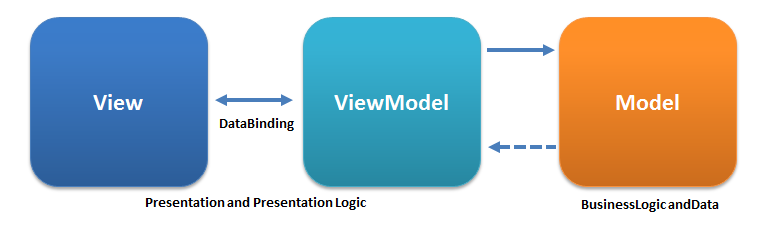
\includegraphics[width=\textwidth]{img/MVVMPattern.png}
        \caption{Three core components of the MVVM design pattern.}
        \label{fig:mvvm_pattern}
        %\source{https://en.wikipedia.org/wiki/Model%E2%80%93view%E2%80%93viewmodel#/media/File:MVVMPattern.png}
        \caption*{Source: \url{https://en.wikipedia.org/wiki/Model\%E2\%80\%93view\%E2\%80\%93viewmodel\#/media/File:MVVMPattern.png}}
    \end{figure}
    
    In the above graph \ref{fig:mvvm_pattern} relations between individual components are presented.
    
    \subsubsection{View}
        View in this case is a synonym of UI (in most cases GUI). Its purpose is to define the appearance of an app -- where and how do buttons look an lay, how the data is presented to the user, which elements are static and which have dynamic binding. As the name suggests, it handles the \textit{view} of the project - what user sees on the screen.
        %
        In the presented application role of the \textit{View} part is taken by a project named \textit{View} \ref{fig:view}.
        
        \begin{figure}[H]
            \centering
            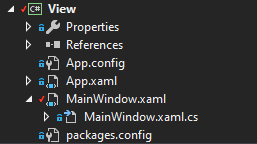
\includegraphics{img/view.png}
            \caption{\textit{View} project seen from Solution Explorer.}
            \label{fig:view}
        \end{figure}
        
        This project \ref{fig:view}, based on Visual Studio 2019 default project \textit{WPF App (.NET Framework)} \ref{fig:view_wpfApp} is the only non-F\# part of the MARS App as, for the time being (December 2020), there is no dedicated project in the F\# language that would, by default, be compatible with MVVM architecture and XAML markup language for presenting the view. Therefore few lines of C\# code needed to be added in order to bind successfully View project with ViewModel one.
        
        \begin{figure}
            \centering
            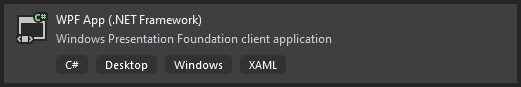
\includegraphics{img/view_wpfApp.png}
            \caption{Default Visual Studio 2019 project used for writing the \textit{View} part of an app.}
            \label{fig:view_wpfApp}
        \end{figure}

    \subsubsection{Model}
        \textit{Model} section handles business logic and data of the app. It is an inherent entity that could be reused in other applications. It is a significant advantage of the MVVM architectural pattern -- reusability of code is supported at the conceptual level of the design pattern.
        
        This time \textit{Model} project \ref{fig:model_VS19Project} is solely an F\# project that targets .Net Framework 4.6.1.
        \begin{figure}[H]
            \centering
            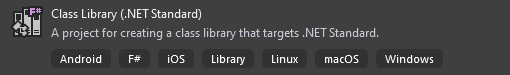
\includegraphics{img/model_VS19Project.png}
            \caption{Default Visual Studio 2019 project used for writing the \textit{Model} part of an app.}
            \label{fig:model_VS19Project}
        \end{figure}
        
        In here it is useful to remind that whenever there is no valid reason to use \textit{.NET Core} over \textit{.NET Framework}, one should always opt for the latter. \textit{.NET Core} is used when multi-platform approach is expected, but if the app is destined for Microsoft Windows system then, the amount of libraries available on \textit{.NET Standard} is vastly higher.
        
        \begin{figure}[H]
            \centering
            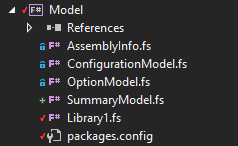
\includegraphics{img/model.png}
            \caption{\textit{Model} project seen from Solution Explorer.}
            \label{fig:model}
        \end{figure} 
        
    \subsubsection{ViewModel}    
        Last but surely not least the \textit{ViewModel} serves a role of a so-called \textit{bridge} between \textit{View} and the \textit{Model}. It binds the graphical presentation of the components with hidden back-end logic. It must hold a reference to the \textit{Model} project of the solution. It is extremely important for the programmer to design proper updates of data presented in corresponding graphic fields. \textit{INotifyPropertyChanged} interface is perfect for this purpose. It makes sure no change in the data filed will go unnoticed if it is able to see it anywhere in the app by the user.
        
        It consists of multiple files responsible for specific purposes, all starting with line:
        
        \begin{lstlisting}[language=FSharp, label={lst:model1}, caption=F\# all \textit{ViewModel} project components beginning.]
            namespace ViewModel
            // lines of code
        \end{lstlisting}
        %
        Alternative syntax could be using F\# \textit{module} declaration what is rather more common nowadays that OOP-resembling \textit{namespace} like so:
        %
        \begin{lstlisting}[language=FSharp, label={lst:model2}, caption=F\# alternative example \textit{ViewModel} project component beginning.]
            module MARSApp.ViewModel.ConfigurationViewModel
            open MARSApp.ViewModel.ViewModelBase
            open MARSApp.Model.ConfigurationModel
            // lines of code
        \end{lstlisting}
        %
        Although the difference and these code fragments \ref{lst:model1} \ref{lst:model2} may seem unimportant, there is a tremendous reason behind choosing the first one -- since the project contains GUI written in XAML there is need to specify in the view where certain properties can be found. It turns out there is a major problem if the properties lay hidden inside a module. When they are presented in a namespace it is easier to bind them with XAML as it is adapted to receive a \textit{namespace} declaration in the \textit{Window} heading:
        %
        \begin{figure}[H]
            \centering
            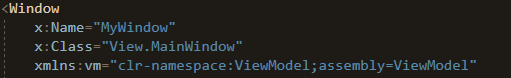
\includegraphics{img/viewmodel_namespace.png}
            \caption{Fragment of file \textit{MainWindow.xaml} showing \textit{namespace} reference.}
            \label{fig:viewmodel_namespace}
        \end{figure}
        %
        The reference would be much harder to achieve if \textit{module} approach was used.
        %
        For the sake of implementing \textit{ViewModel} in this example the same default VS19 project was used as in \textit{Model} project.
        
        \begin{figure}[H]
            \centering
            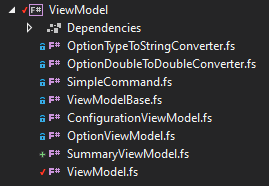
\includegraphics{img/viewmodel.png}
            \caption{\textit{ViewModel} project seen from Solution Explorer.}
            \label{fig:viewmodel}
        \end{figure} 
    
\subsection{XAML}
    \textit{XAML} stands for Extensible Application Markup Language and belongs to declarative markup language group. It is used in \textit{WPF} (\textit{Windows Presentation Forms} -- User Interface framework for creating desktop client applications, for more detail go there \cite{wpf}) for separating between how an application looks like and how it behaves (see here how xaml works \cite{how_xaml_works}) (both the GUI and its behavior were created in the same language). \textit{XAML} is an subset of \textit{XML}, because every \textit{XAML} file is as well a \textit{XML} file, but not every \textit{XML} file is a \textit{XAML} file.
    
    \textit{XAML} may resemble \textit{HTML}, although the idea behind those two is utterly different -- by comparing \textit{XML} to \textit{HTML} one can observe that:
    \begin{itemize}
        \item \textit{XML} is a markup language much like \textit{HTML} but \textit{HTML} was designed to display data while \textit{XML} to carry it.
        \item \textit{HTML} tags (such as: <p>, <h1>, <table>, etc.) are predefined while \textit{XML} ones are created at the moment by the programmer.
        \item \textit{HTML} allows small coding errors and is case insensitive in opposition to \textit{XML}.
    \end{itemize}
